\documentclass[12pt]{article}
\usepackage{cite}
\usepackage{graphicx}
\usepackage{geometry}
\usepackage{float}
\usepackage{multicol}
\usepackage{amsmath}

\geometry{left=2.0cm,right=2.0cm,top=2.5cm,bottom=2.5cm}

\title{
    \textbf{\Huge ECE385} \\
    \huge Fall 2020 \\
    \huge Experiment 2 \\[120pt]
    \textbf{\Huge Data Storage} \\[120pt]
    }

\author{
    \large Name: Zhou Qinren \\ 
            \quad\qquad Zhang Yichi \\
    \large Lab Section: LA3 \\
    \large TA's Name: Yu Yuqi
    }

\date{Sept. $24^{th}$ 2020}

\begin{document}
\setlength{\parindent}{0pt}
\maketitle
\newpage

\section{Introduction}
Our circuit serves as a random-access memory (RAM). It can store data into some individually identified locations, which can be accessed by specifying a unique address (bit-string). Our design contains four words, using 2-bit of each word. The fundamental elements in our design are registers and control logic. The former one is used to store the data, and the latter one
realizes read/write operations.

\section{Operation of the Memory Circuit}
\subsection{\textbf{Addressing}}
Addressing is implemented by a counter and a comparator. The SAR here is not a unique space in the memory. Instead, each address is mapped to a unique state of a 2-bit counter and each state occupies one space in the shift register which is the memory in our design. Therefore, only when the comparator outputs a 1 indicating that the address matches with the counter's state, we know we are on the correct address and it is valid to fetch or write. The circuit commits a read from the input switches when the LDSBR is high. The circuit commits a write to the output register when the STORE is high.

\subsection{\textbf{Write Operation}}
In order to perform a write operation, we first ensure that all the switches are off and then turn on the LDSBR switch. According to the control logic, the 3 to 1 mux will load the data we want to write into the SBR (Storage Buffer Register) for the next cycle. Then we turn off the LDSBR, set the SAR1 and SAR0 and turn on the STORE. After waiting several clock cycles for the counter to be matched up with the SAR signal, the control logic will send a select signal to the 2 to 1 mux to let the new data from the SBR flow in and cover the original one at the next clock cycle.

\subsection{\textbf{Read Operation}}
In order to perform a read operation, we first ensure that all the switches are off, set the SAR1 and SAR0 and then flip the switch to turn on the FETCH signal. After waiting several clock cycles for the counter to be matched up with the SAR signal, the control logic will send a select signal to the 3 to 1 mux to let the data flow out of the shift register and be stored in the SBR at the next colck cycle.

\section{Written Description and Block Diagram of Memory Circuit Implementation}
\subsection{\textbf{High-Level Description}}
To perform the addressing, write and read operations and better organize the circuit, we divide our design into three parts: memory unit, buffer unit and control logic. The memory unit consists of a 2 to 1 mux to select whether to write new data in or hold the original data and a 4-bit shift register to store the words. The buffer unit consists of an SBR to store one word that is going to be read out to the output or written into the memory shift register and a 3 to 1 mux to select whether to store the data from the memory shift register or from the inputs DIN or from the original SBR into the SBR. The control logic consists of a combinational circuit that takes in the inputs FETCH, STORE, SAR1, SAR0 and LDSBR and outputs a 1-bit select signal to the memory unit and a 2-bit select signal to the buffer unit. The detailed logic will be presented in the following section.

\subsection{\textbf{High-Level Block Diagram}}
\begin{figure}[H]
    \centering
    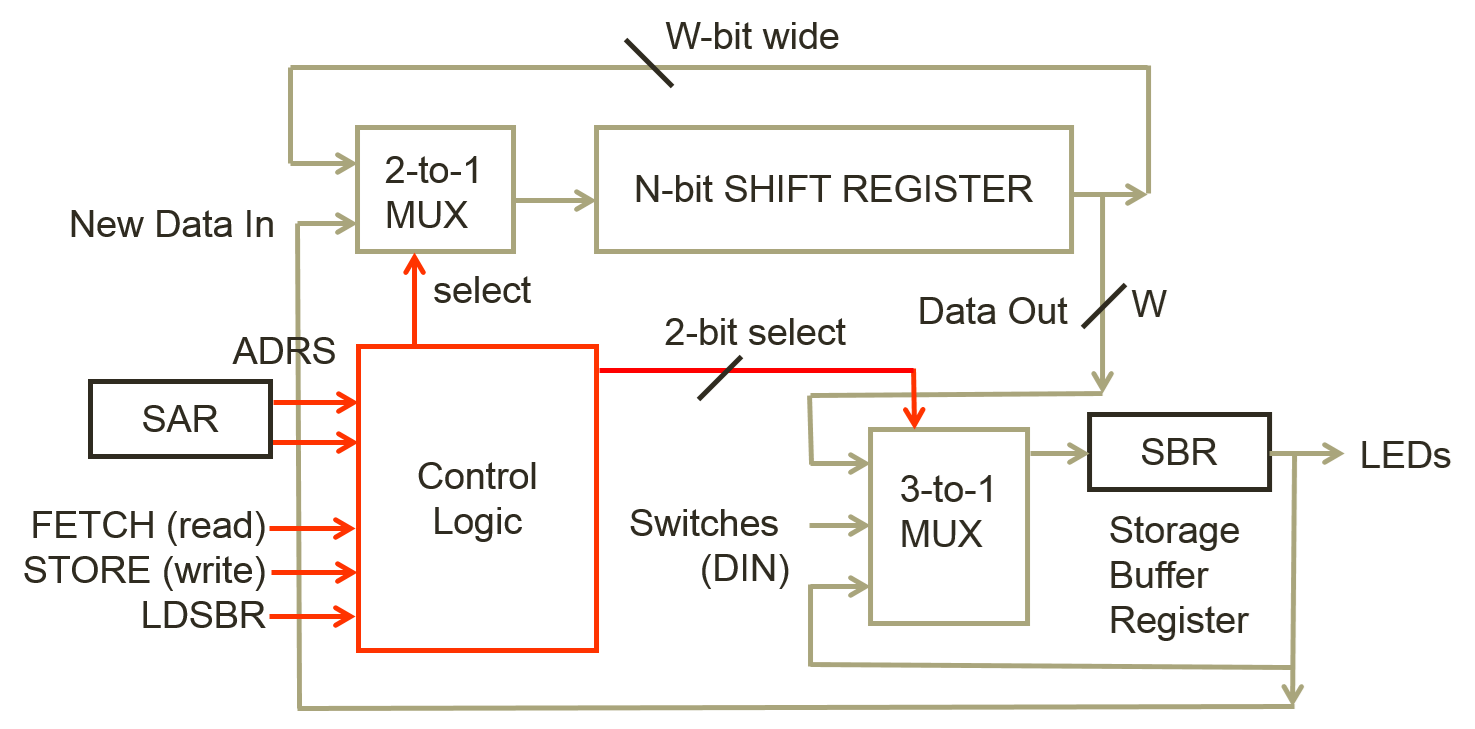
\includegraphics[scale=0.5]{high_level_diagram.png}
    \caption{High-level block diagram \cite{GG}}
\end{figure}

\section{Control Unit}
\subsection{\textbf{Written Description}}
Our control unit consists of two separate parts, an address unit and an output logic. \\

The first part, the address unit, determines whether the current address is the same as the input address (SAR). The comparation is implemented by a 4-bit counter and a comparator. We only make use of the two least significant bits of counter to keep counting. If the input address (SAR) is equal to the current counter value, then the comparator will output a signal EQUAL, which indicates the current location in register is exactly the location we want to manipulate. \\

The second part is a just a bunch of logic gates. The logic circuit accepts the following input: FETCH, STORE, LDSBR and EQUAL (from address unit), and generates SELECT outputs to the register unit and buffer unit. In short, the logic circuit receives instructions from users such as FETCH or STORE, then it outputs the select signal to the registers and SBR to have them worked as desired. The SELECT signal to the register unit contains only one bit, since the receiver is a 2-to-1 mux, while the SELECT signal to the buffer unit contains two bits, which are denoted as SELECT0 and SELECT1. We used a k-map to simplify the logic.

\subsection{\textbf{Block Diagram}}
\begin{figure}[H]
    \centering
    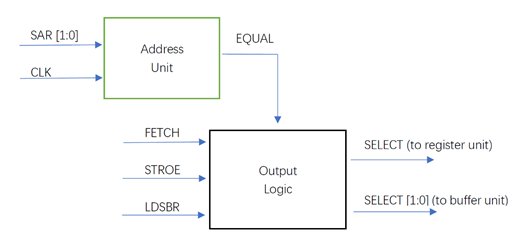
\includegraphics[scale=1.2]{block_diagram.png}
    \caption{Block diagram}
\end{figure}

\section{Design Steps Taken and Detailed Circuit Schematic}
\subsection{\textbf{Truth Tables}}
\begin{table}[H]
    \centering
    \resizebox*{7cm}{3cm}{
    \begin{tabular}{ccc}
    STORE & EQUAL & SELECT \\ \hline
    0     & 0     & 0      \\
    0     & 1     & 0      \\
    1     & 0     & 0      \\
    1     & 1     & 1     
    \end{tabular}
    }
    \caption{Truth table of the 1-bit select signal for memory unit}
\end{table}
$$SELECT=STORE\cdot EQU\!AL$$

\begin{table}[H]
    \centering
    \resizebox*{13cm}{6cm}{
        \begin{tabular}{ccccc}
            LDSBR & FETCH & EQUAL & SELECT1 & SELECT0 \\ \hline
            0     & 0     & 0     & 0       & 0       \\
            0     & 0     & 1     & 0       & 0       \\
            0     & 1     & 0     & 0       & 0       \\
            0     & 1     & 1     & 1       & 0       \\ \hline
            1     & 0     & 0     & 0       & 1       \\
            1     & 0     & 1     & 0       & 1       \\
            1     & 1     & 0     & x       & x       \\
            1     & 1     & 1     & x       & x      
            \end{tabular}
    }
    \caption{Truth table of the 2-bit select signal for buffer unit}
\end{table}
$$
\begin{aligned}
    SELECT1&=FETCH\cdot EQU\!AL \\
    SELECT0&=LDSBR
\end{aligned}
$$

\subsection{\textbf{Detailed Circuit Schematic}}
The overall circuit schematic. It consists of three parts, the control logic, the memory unit, and the buffer unit. The control logic deals with the user instruction, the memory unit stores data and the buffer unit load the input data or retrieve data from the memory.
\begin{figure}[H]
    \centering
    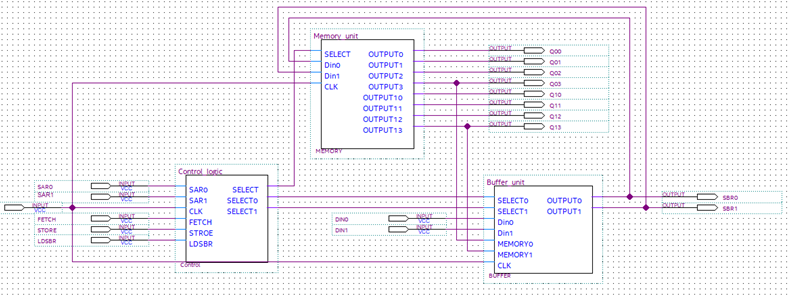
\includegraphics[width=15cm]{overall_circuit.png}
    \caption{Overall circuit}
\end{figure}
SELECT [1:0] is generated by control logic, which is used to select the input to the SBR (flip-flop). The output of the SBR is connected to the memory unit and SBR itself. 
\begin{figure}[H]
    \centering
    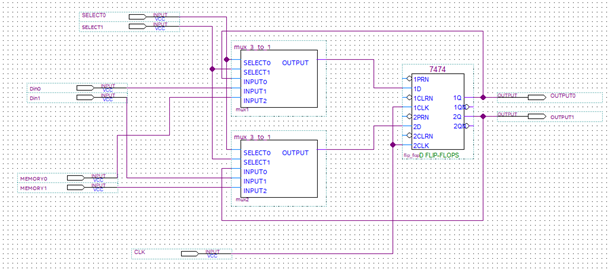
\includegraphics[width=15cm]{buffer_unit.png}
    \caption{Buffer unit}
\end{figure}
SELECT signal is generated by control logic and is used to select the input to the shift register. Since we are designing a 2-bit register, we combined two 74194 into a 2-bit shift register, as shown below. The input to the shift register is the output of the 2-to-1 mux.
\begin{figure}[H]
    \centering
    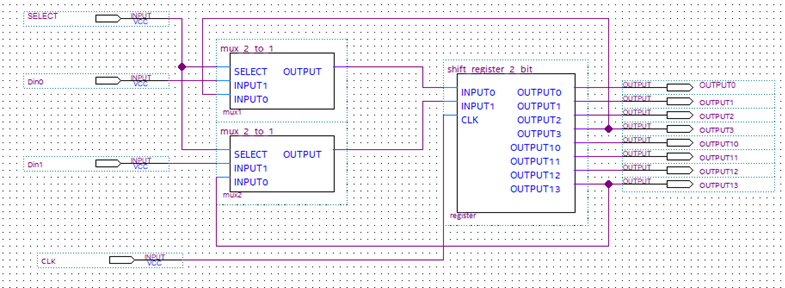
\includegraphics[width=15cm]{memory_unit.png}
    \caption{Memory unit}
\end{figure}
\begin{figure}[H]
    \centering
    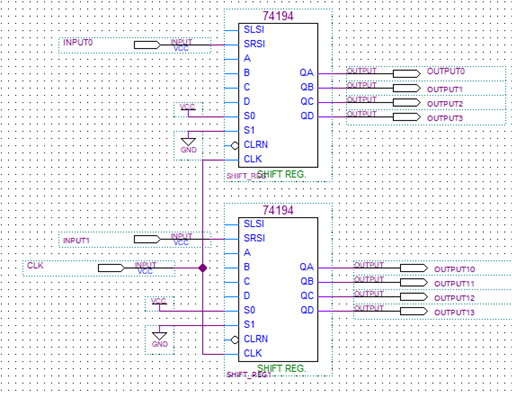
\includegraphics[width=15cm]{shift_register.png}
    \caption{Shift registers}
\end{figure}
\begin{figure}[H]
    \centering
    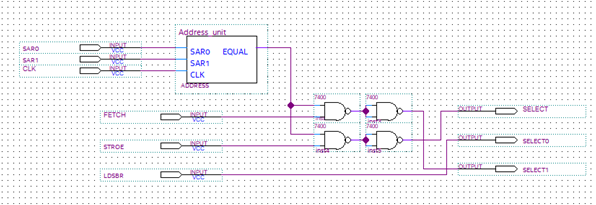
\includegraphics[width=15cm]{control_logic.png}
    \caption{Control logic}
\end{figure}
The address unit compares the current location in register and the input address, then output a signal to indicate whether we are accessing the desired location. 
\begin{figure}[H]
    \centering
    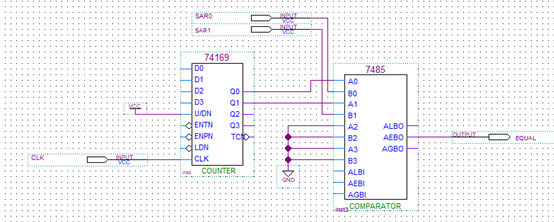
\includegraphics[width=15cm]{address_unit.png}
    \caption{Address unit}
\end{figure}
Additional: \\
We constructed 2-to-1 mux and 3-to-1 mux on our own. The following are the logic circuits in the gate-level. 
\begin{figure}[H]
    \centering
    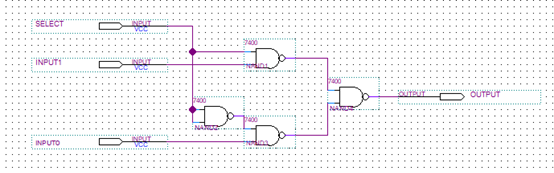
\includegraphics[width=15cm]{2to1mux.png}
    \caption{2 to 1 MUX}
\end{figure}
\begin{figure}[H]
    \centering
    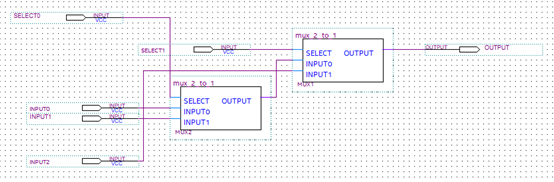
\includegraphics[width=15cm]{3to1mux.png}
    \caption{3 to 1 MUX}
\end{figure}

\section{Description of All Bugs Encountered and Corrective Measures Taken}
When we design this project, we found it hard to connect the wires at first, because there were many gates and chips, making the whole screen a completely mess. Then we adapted the hierarchy strategy. With the help of abstraction, we make our design clear and simple. \\

Another problem is that we did not use flip-flop to construct the SBR at first. We designed a combination logic for the buffer unit, instead of a sequential logic. This caused some unpredicted bugs, and then we changed the circuit into a sequential one. 


\section{Conclusion}
\subsection{\textbf{Summarization}}
In this lab, we learn to use Quartus to design and construct a simple 2-bit 4-word memory with basic store, read and write operations. Also, it is our first time to build such a complicated circuit with several parts, each of which has its own functionality and works independently. It is vital to organize and divide them into modules to make our design clearer and easier to debug.

\subsection{\textbf{Answers to Pre-Lab Questions}}
Question: The registers must be shifted on each clock pulse. The clock must run continuously – do not gate the clock (this is bad practice in digital design, why?) \\

Answer: Because gating the clock will cause delays that might lead to glitches and make some of the chips asynchronized which then results in false outputs. \\

Question: Only the clock input needs to be de-bounced to step through your circuit (why?). \\

Answer: In real implementation, the signal FETCH, STORE, LDSBR are controlled by switches. Flipping switches might cause glitches due to contact bounce because the contact points are not so ideal that may not stabilize immediately. In a short arrange of time, there will be unexpected bounce between 0 and 1 which might trigger some chips. Thus, we have to and only need to debounce the clock signal since once the clock signal is debounced the chips will not be triggered and the other bounces will not influence the output.

\subsection{\textbf{Answers to Post-Lab Questions}}
Question: What are the performance implications of your shift register memory as compared to a standard SRAM of the same size? \\

Answer: To fetch data from or write data into particular addresses, the shift register we build has to wait several clock cycles for the counter to be matched with the address we desire. While a standard SRAM uses muxes to locate the particular address which is much more fast than our design. That is to say, our design is only feasible when there is a small number of addresses. Otherwise, it will take a large amount of time to fetch or write. \\

Question: What are the implications of the different counters and shift register chips, what was your reasoning in choosing the parts you did? \\

Answer: The counter we need is a 2-bit counter which can be built by taking the first 2 bits from the 4-bit counter in our lab kit. Then we have choices SN7493 (4-bit Ripple Counter), SN74LS169A (4-bit Synchronous Up-Down Counter) and SN74193 (4-bit Synchronous Up-Down Counter). We choose SN74193 because it is synchronous, stable and easier to build. SN7493 needs two different clock cycles. SN74LS169A needs two enable signals. For shift register chips, there are only two choices in the lab kit, SN7495 (4-bit Parallel-Access Shift Registers) and SN74LS194A (4-bit Bidirectional Universal Shift Register). Both of them work well. We choose the latter one and use its shift right mode and serial input since we only manipulate 1 bit data per 1 shift register in this lab.

\newpage
\bibliography{lab2_ref}
\bibliographystyle{ieeetr}
\end{document}